\documentclass{article}
\usepackage[utf8]{inputenc}
\usepackage{titling}
\usepackage{graphicx}
\usepackage[dvipsnames]{xcolor}
\usepackage[colorlinks=true,linkcolor=darkgray, urlcolor =gray]{hyperref}
\usepackage[spanish]{babel}
\DeclareUnicodeCharacter{301}{~}
\usepackage{url}
\usepackage{graphicx}
\usepackage{caption}
\usepackage{subcaption}
\DeclareUnicodeCharacter{202F}{\,}
\DeclareUnicodeCharacter{20AC}{\euro{}}
\usepackage{float}
\usepackage[shortlabels]{enumitem}


\title{Caso práctico: segunda entrega}
\author{Grupo O\\ Álvaro Fernández Palma\\ Alina Altynguzhina\\ Iman Hasnaouia Meskini\\ Cristina Díaz García\\ \\3º de Ingeniería Informática}
\date{Diciembre 2018}

\renewcommand\maketitlehooka{\null\mbox{}\vfill}
\renewcommand\maketitlehookd{\vfill\null}


\begin{document}

\addcontentsline{toc}{section}{Índice general}

\begin{titlingpage}
\maketitle

\end{titlingpage}

\newpage

\tableofcontents

\newpage

\section{Introducción}

\subsection{Descripción de la organización y de su actividad principal} 

La empresa sobre la que vamos a trabajar se llama Puente. \textcolor{Red}{Es una pyme de 9 trabajadores.} La razón por la que la hemos escogido es que uno de nuestros compañeros trabaja allí. Se trata de una empresa que presta servicios a otras empresas respecto a publicidad: creación de marca (branding), storytelling, programación web y tienda online, redes sociales, videos/spots, resumiendo, todo lo relacionado con marketing. Con el objetivo de dar una visibilidad a las empresas de cualquier tamaño y llegar a cualquier público con eficacia. Entre los clientes se encuentran: Adidas, Suzuki, Ubago, Malaga Wagen, etc

\subsection{Breve resumen del trabajo realizado}

Nuestro trabajo consistió en hacer un informe sobre una empresa relacionándolo con todo lo aprendido en las clases.  Se han buscado empresas y propuesto alternativas, y al final se escogió una empresa en la que uno de nuestros miembros del grupo es trabajador.

\textcolor{Red}{Al principio de esta memoria, apartado 2, hablamos de conceptos generales y vistos en clase. Identificamos los sistemas físico, directivo y de información de la organización describiendo las actividades que se hacen en cada departamento. Tras esto hablamos de niveles existentes de sistemas de información en la organización, tanto de operativo, táctico, como de estratégico. Describimos los programas y hablamos sobre el uso que se le da en cada departamento de la empresa. Aparte mencionamos los servicios que coge prestados la empresa de algunas plataformas.}  

\textcolor{Red}{En siguiente apartado 3 se habla de infraestructuras TIC: el hardware que se utiliza en la empresa, programas y plataformas.} 

\textcolor{Red}{El apartado 4 trata sobre la planificación de sistemas de información. Hablamos sobre objetivos a medio-largo plazo de la empresa y los sistemas de información que se utilizan para poder llegar a esos objetivos. Se comenta la situación actual de SI de esta organización, por ello hablamos de esos softwares y clasificamos de forma funcional.} 

\textcolor{Red}{A continuación, se analizan esos sistemas donde finalmente se proponen dos softwares para gestión comercial. Se crean y se describen los criterios para poder calificarlos y de esta manera escoger el mejor. Mostramos tablas de modelo de calificación y coste total de propiedad de ambos programas. Y basándonos en resultado salido en modelo de calificación, escogemos el mejor software para gestión comercial y planteamos los cambios que se producirían al implantar la opción ganadora.} 

\textcolor{Red}{Analizamos aspectos de Almacén en esta empresa para poder plantear nuevas opciones y optimizar el negocio. }  

\textcolor{Red}{Lo mismo hacemos con comercio electrónico, donde analizamos la situación actual, proponiendo criterios de calificación para opciones: al tener la tienda online o no tenerla. Y hablamos sobre la opción ganadora si llegáramos a implantarla y los cambios que se producirían.}  

\textcolor{Red}{A continuación, se habla sobre CRMs. Se comenta sobre lo que utiliza la empresa: softwares tipo CRM. Y se proponen tres programas con sus modelos de calificación correspondientes y costes de propiedad. Se elige según lo que haya salido en el resultado y se comentan los cambios que implicaría al implantar este software.}  

\textcolor{Red}{Y finalmente, este apartado se acaba con el archivo electrónico. Tratamos el tema de gestión de documentos y almacenamiento de los archivos a largo plazo. Se comenta si hay algún software en la empresa que se encargue de estas funcionalidades, y si resultaría de utilidad implantar una opción u otra, o ambas.  Al escoger una de estas opciones mencionadas anteriormente se proponen softwares. A continuación, vienen las tablas donde tenemos criterios descritos, modelo de calificación y coste total de propiedad de esos programas. Y el resultado final con los cambios que se producirían en la empresa al escoger un programa ganador.}

\textcolor{Red}{El apartado 6 trata sobre la integración de sistemas de información con programas actuales que se utilizan en la empresa. Si sería posible hacerlo, qué programas se integrarían.}  

\textcolor{Red}{En el apartado 7, se habla sobre los sistemas de flujo de trabajo de la empresa. Se crean diagramas con ayuda de Bizagi para poder explicar con más facilidad los tres flujos de trabajo que se hayan elegido.}

\textcolor{Red}{En el apartado 8, hablamos sobre propuestas innovadoras de sistemas de información para esta empresa.}

\textcolor{Red}{En el siguiente apartado 9, tenemos tablas de tareas que cada miembro ha desempeñado con su estimación temporal. Y otra tabla que era de la primera entrega.}

\textcolor{Red}{Finalmente, en apartado 10, tenemos la conclusión, donde hablamos sobre el efecto que tendría en la empresa al implantar nuevas opciones comentadas en este documento: sus pros y contras, y si finalmente merece la pena o no.} 

\section{Conceptos generales}

\subsection{Identificar el sistema físico, directivo y de información de la organización. Describirlos desde el punto de vista funcional}

\textcolor{Red}{En la empresa elegida, nuestro sistema físico se compone de los siguientes elementos:}

\begin{itemize}
\item \textcolor{Red}{\textbf{Departamento de diseño:} Diseñan tanto logos como el layout de las páginas web.}
\item \textcolor{Red}{\textbf{Departamento de información:}  Crean infografías y gestionan la información de la que la empresa dispone. También organizan los proyectos y su estado (deadlines y progreso). Desarrollan la actividad a la que la empresa se dedica: desarrollar software.}
\item \textcolor{Red}{\textbf{Departamento de captación o comercial:} Tratan con los clientes, preparan las reuniones con ellos y buscan nuevas empresas con las que trabajar.}
\item \textcolor{Red}{\textbf{Departamento de redes:} Promocionan la actividad de la empresa en redes sociales y monitorizan el impacto que esta promoción tiene sobre el público general.}
\item \textcolor{Red}{\textbf{Departamento de contabilidad:} Llevan el control de los gastos e ingresos que la empresa sufre.}
\end{itemize}

\textcolor{Red}{El sistema directivo, por otra parte, tiene las siguientes partes:}

\begin{itemize}
\item \textcolor{Red}{\textbf{Dirección Ejecutiva:} Lidera la empresa y supervisa que todo funcione. También coordina al resto de directivos.}
\item \textcolor{Red}{\textbf{Dirección de Marketing:} Crea e implementa las estrategias que se implementarán en el mercado, aportando valor. También comprueba la situación de la empresa en el mercado: si crece o disminuye y sus posibilidades de seguir creciendo, optimizándolas.}
\item \textcolor{Red}{\textbf{Dirección de comunicación:} Diseña la estrategia de promoción que tendrá la empresa: redes sociales, web, incluso periódicos, radio o televisión si se viera conveniente. Realiza estudios de las analíticas de impacto para decidir esta estrategia.}
\item \textcolor{Red}{\textbf{Dirección de Información:} Planifica los procesos y canales de comunicación para una información fluida y eficiente en la empresa, de modo que el conocimiento, la experiencia y la creatividad del resto de personas del equipo fluyan.}
\item \textcolor{Red}{\textbf{Dirección del área tecnológica:} Gestiona los recursos tecnológicos para cumplir los objetivos, mientras supervisa que éstos se cumplan, tanto en calidad como en fecha.}
\item \textcolor{Red}{\textbf{Dirección Financiera:} Aporta el criterio financiero: regula los gastos e ingresos que la empresa tiene, intenta maximizar la liquidez de la empresa. Es quien estudia el mercado para saber en qué invertir.}
\end{itemize}

\textcolor{Red}{El sistema de información es, por otra parte:}

\begin{itemize}
\item \textcolor{Red}{El software usado en la empresa, que se detalla posteriormente, va desde software para llevar la contabilidad o las analíticas de las redes sociales, pasando por diseño y edición o incluso ofimática, hasta software usado para el desarrollo.}
\end{itemize}

En esta empresa se utilizan unos u otros programas dependiendo de los departamentos. A continuación, enumeraremos los programas utilizados en cada departamento, y tras eso, haremos una descripción de cada software.  

\begin{itemize}
\item \textbf{En departamento de diseño:} Photoshop, Illustrator, InDesign 
\item \textbf{En departamento de información:} Photoshop 6, Adobe Dreamweaver, FileZilla, Trello, HTML5, PHP 7.3 
\item \textbf{En departamento de captación o comercial:} Trello, Microsoft Word, Microsoft Excel y Microsoft Power Point.
\item \textbf{Departamento de redes:} Pixel, Business Facebook, Google Adds, Microsoft Word, etc. 
\item \textbf{Departamento de contabilidad:} Factual, Plataforma del Banco Santander. 
\end{itemize}

\vspace{5mm}

\textbf{Photoshop}

Photoshop es un editor de gráficos rasterizados desarrollado por Adobe. Sirve para retocar fotografías y gráficos. Y en este caso, en nuestra empresa, sirve para hacer cualquier diseño, ya sea un panfleto, un stand publicitario o diseño web, es decir, todo lo relacionado con una imagen.  

Sus características principales, es que se trabaja en capas. Esto es, cada capa es independiente, se trabaja en ella y no afecta a los demás, a no ser que quieras lo contrario, que también tiene esa funcionalidad. Es muy versátil, por ello es un programa mundialmente conocido, se pueden hacer muchísimas cosas con él. 

Al contrario que otros programas, como por ejemplo CorelDraw, Photoshop es un programa que trabaja en pixeles. Por tanto, es un problema si el trabajo final lo quieres tener muy definido, muy nítido, aunque también depende de cuantos pixeles estemos hablando.  

Es un programa de pago. La última versión es tipo cloud, Adobe CC (que es un paquete que reúne todos los programas de diseño de Adobe), y el pago es mensual. Se puede pagar solo por un programa al mes, o paquete completo.  Nuestra empresa utiliza la versión cloud con el paquete completo. 

\vspace{5mm}

\textbf{Illustrator}

Illustrator es un editor de gráficos vectoriales que trabaja sobre un tablero de dibujo llamado “mesa de trabajo”. Es desarrollado y comercializado por Adobe Systems. Con este programa se puede crear un dibujo artístico y pintura para la ilustración. Los usos que se le dan abarcan distintas áreas como maquetación – impresión, video, publicación web y dispositivos móviles.  

Actualmente, tiene como función única y primordial la creación de material gráfico-ilustrativo altamente profesional basándose para ello en la producción de objetos matemáticos denominados vectores.  

La última versión de Illustrator viene en paquete Adobe Creative Cloud. La empresa Puente tiene la versión cloud, al igual que la de Photoshop, el pago es mensual.

\vspace{5mm}

\textbf{InDesign}

Adobe InDesign (ID) es una \href{https://es.wikipedia.org/wiki/Aplicaci\%C3\%B3n_inform\%C3\%A1tica}{aplicación} para la \href{https://es.wikipedia.org/wiki/Maquetaci\%C3\%B3n\_(edici\%C3\%B3n)}{composición digital de páginas} desarrollada por la compañía Adobe Systems y dirigida a maquetadores profesionales. Sirve para diseñar folletos, panfletos, revistas, periódicos y libros.  

Actualmente, InDesign no es solo una aplicación orientada a la maquetación o trabajo editorial, desde hace ya varias versiones se han incorporado herramientas para crear archivos multimedia, pdf interactivos para páginas web y dispositivos móviles.  

El método de compra es igual al de Photoshop o Illustrator: se paga mensualmente solo el programa o todo. Algunas empresas lo compran para siempre y lo instalan, que sería la versión instalada (o como se dice en inglés “on premise”). En nuestro caso, es de pago mensual.

\vspace{5mm}

\textbf{Adobe Dreamweaver}

Adobe Dreamweaver es un programa que se utiliza para construcción, diseño y edición de sitios, videos y aplicaciones web. Se puede programar en cualquier idioma, pero Adobe Dreamweaver soporta html, css, php, javascript. Lo que queremos decir es que en este programa está implementado el autocompletado y sugerencias con estos lenguajes de programación.  

Lo bueno de este programa es que mientras estás programando, ya estás visualizando como quedaría.  También hay plantillas para agilizar el proceso de diseño. Y además, tiene en cuenta la adaptabilidad para diferentes dispositivos.  

Respecto al pago, es lo mismo que con todos programas de Adobe: se paga mensualmente el programa o la colección entera de programas de Adobe. En este caso, tenemos un programa con el pack completo y pago mensual.  

\vspace{5mm}

\textbf{FileZilla}

FileZilla es un software que te permite conectarte a un servidor utilizando protocolo FTP para transferir archivos, también se utiliza con cifrado FTPS y SFTP.  

Algunas de las características:  

\begin{itemize}
\item es compatible con IPv6, que es la última versión del protocolo de Internet.
\item soporta para reanudar, lo que significa que el proceso de transferencia de archivos se puede pausar y continuar.
\item interfaz de usuario con pestañas para realizar múltiples tareas, para permitir navegar por más de un servidor o incluso transferir archivos simultáneamente entre múltiples servidores.
\end{itemize}      

La empresa lo utiliza para hostear el servidor de pruebas donde ellos programan.   

El programa es multiplataforma, tiene versiones servidor y cliente, y es de código abierto y libre.

\vspace{5mm}

\textbf{Trello}

Trello es un software de gestión de proyectos con interfaz web, cliente para Android y iOS para organizar proyectos. Empleando el sistema \href{https://es.wikipedia.org/wiki/Kanban}{kanban} (letrero o valla publicitaria en japonés), para el registro de actividades con tarjetas virtuales organiza tareas, permite agregar listas, adjuntar archivos, etiquetar eventos, agregar comentarios, colgar imágenes, enlaces y compartir tableros. 

La empresa lo usa para intercomunicar los departamentos y organizar los flujos de trabajo. Se sincroniza en todos los dispositivos y es gratuito.

\vspace{5mm}

\textbf{HTML5}

Es un lenguaje de marcas de hipertexto para estructurar y presentar contenido en la Web.  Es la quinta versión de html estándar. HTML5 tiene dos variantes de sintaxis: una “clásica”, HTML, conocida como HTML5, y una variante \href{https://es.wikipedia.org/wiki/XHTML}{XHTML} conocida como sintaxis XHTML5 (XML). Se introducen herramientas notables como etiquetas que permiten la publicación de archivos de audio y video con soportes de distintos codecs; tags para que los usuarios dibujen contenidos en 2D y 3D; cambios en los llenados de formularios; y una web semántica mucho mejor aprovechada. Básicamente, se puede crear páginas web dinámicos e interactivos sin el uso de Flash. 

\vspace{5mm}

\textbf{PHP 7.3}

Es un lenguaje de programación de propósito general de código del lado del servidor orientado a desarrollo web de contenido dinámico con acceso a bases de datos.  Ejemplos de usos: recopilación de datos de formularios, generación de páginas con contenidos dinámicos, enviar o recibir cookies. Con PHP no se está limitado a generar HTML. Entre las capacidades de PHP se incluyen la creación de imágenes, ficheros PDF e incluso películas Flash (usando libswf y Ming) generadas sobre la marcha. 

Hace poco la empresa lo actualizó a la última versión, php 7.3, que salió este mes diciembre de 2018.

\vspace{5mm}

\textbf{Microsoft Word}

Es un programa orientado a procesamiento de textos. Fue creado por Microsoft y está integrado en paquete ofimático, Microsoft Office. Permite crear documentos (de texto, gráficos, tablas, cartas, etc) que se pueden guardar en múltiples formatos, entre ellos doc que es el formato propio de Word.  

Actualmente, la última versión es cloud, Office 365, integrado por más programas de Microsoft. Para obtener Office 365 hay que pagarlo anualmente.  También se tiene la opción de comprarlo en único pago y disfrutar de Word, Excel y PowerPoint para siempre, pero no en versión cloud, sino que instalándolo.   

La empresa utiliza la versión cloud con el pago anual.  

\vspace{5mm}

\textbf{Microsoft Excel}

Es un programa ofimático de Microsoft, al igual que Word está incluido en el paquete.  

Es una aplicación de hojas de cálculo utilizada en tareas financieras y contables, con fórmulas, gráficos y un lenguaje de programación. Excel permite a los usuarios elaborar tablas y formatos que incluyan cálculos matemáticos mediante fórmulas, además de poder utilizar elementos denominados funciones (fórmulas preconfiguradas). Respecto a la programación, se pueden integrar macros en los archivos de Excel que automatizan tareas de usuario.  

El pago es el mismo que con Word: se paga anualmente o en un único pago. Esta última opción te permite obtenerla de forma local, y no en la nube. En la empresa lo paga anualmente. 

\vspace{5mm}

\textbf{Microsoft Power Point}

Es un programa ofimático de Microsoft, integrado en paquete Office. Permite crear presentaciones con texto esquematizado, así como presentaciones en diapositivas, animaciones de texto e imágenes prediseñadas o importadas desde imágenes de la computadora. Se le pueden aplicar distintos diseños de fuente, plantilla y animación. 

El pago se realiza anualmente con Office 365, a no ser que quieras tenerlo para siempre y de forma instalada.  

La empresa lo tiene en versión nube.

\vspace{5mm}

\textbf{Facebook Pixel}

Es una herramienta que ayuda a medir y optimizar campañas publicitarias en plataforma de Facebook. Facebook Píxel permite medir las conversiones (acciones claves dentro de la estrategia de marketing definidos por la empresa) con el fin de monitorizar y analizar las acciones que realizan los usuarios en página web de la empresa tras ver su anuncio publicado en Facebook. Este código realiza un seguimiento de la conversión y proporciona datos para calcular el retorno de la inversión, además de permitir la optimización de los anuncios. En resumen, es un fragmento de código javascript que insertamos en nuestra página web con el fin de realizar el seguimiento de las conversiones que podrían ser siguientes:  

\begin{itemize}
\item Artículos agregados al carrito de la compra
\item Artículos agregados a la lista de deseos
\item Información de pago agregada
\item Pago iniciado 
\item Compra de producto 
\item Búsqueda en la página web 
\item Contenido visualizado
\end{itemize}   

\vspace{5mm}

\textbf{Business Facebook}

Son herramientas de marketing para ver los comportamientos de los clientes, sacando los datos y midiéndolo todo con el fin de obtener estadísticas y analizar la información para luego convertirlo en conocimiento con valor y aplicarlo en siguientes anuncios con el fin de obtener más público y más clientes. 

\vspace{5mm}

\textbf{Google Ads}

Es una herramienta de Google que te posibilita publicar un anuncio en los resultados de búsquedas de Google. Es para dar visibilidad a tu empresa, sabiendo que muchísima gente utiliza el buscador Google. Se paga solo si alguien visitó tu página web. 

\vspace{5mm}

\textbf{Contabilidad}

Todo se hace con la ayuda de Excel y a través de plataforma de Santander. Se añaden en las tablas los datos que se rellenan en plantillas y se calculan automáticamente. Y todo eso también se envía a la plataforma de Santander. 

\subsection{Niveles de utilización de los sistemas de información existentes en la organización: operativo/transaccional, táctico y estratégico.}

\begin{itemize}
\item \textcolor{Red}{\textbf{Operativo/transaccional:} todos aquellos que usan en el día a día los trabajadores de menor rango: Photoshop, HTML5, el paquete ofimático de Microsoft...}\\
\textcolor{Red}{Un ejemplo del nivel transaccional sería la utilización del recurso de HTML5 por parte del departamento de programación para desarrollar una nueva página web o el uso de Photoshop por parte del departamento de diseño para la creación de un logo empresarial para un cliente.}
\item \textcolor{Red}{\textbf{Táctico:} Aquellos que ponen en práctica los planes y metas establecidos: Trello, Google Ads, la plataforma del banco Santander...}\\
\textcolor{Red}{Un ejemplo del nivel táctico sería llevar un registro de la continuidad y el estado actual de los proyectos que se están llevando a cabo en la empresa, mediante la plataforma Trello, para que todos los departamentos puedan comunicarse los unos con los otros.}
\item \textcolor{Red}{\textbf{Estratégico:} Los usados para definir las metas a largo plazo: Factual, plataforma del banco Santander...}\\
\textcolor{Red}{Un ejemplo a nivel estratégico sería reducir la dependencia de la empresa frente a clientes pequeños y apostar por clientes más competitivos y grandes, obteniendo así una cantidad de clientes muy parecida a la actual pero el ganancial sería mucho más alto, ya que el grueso de trabajo sería equiparable al de hoy en día, pero dichos clientes aportarían mayores beneficios a la empresa.}
\end{itemize}

\section{Infraestructura de TIC}

\subsection{Hardware}

\textcolor{Red}{En dicha empresa hay un total de 9 ordenadores y 1 servidor con 4 discos duros externos.}

\subsection{Software}

\textcolor{Red}{8 de los 9 ordenadores usan el sistema operativo MAC y, el dedicado a la facturación y contabilidad, usa Windows. Mientras que el servidor se usa para el mantenimiento de las páginas creadas ya a los clientes, crear nuevas páginas y poder tener tantas copias de seguridad como se quiera ante la necesidad de hacer algún ROLL BACK (se borrase o sobrescribiera algún archivo erróneamente, por ejemplo).}

\textcolor{Red}{\textbf{Componentes de la infraestructura de TI}} 

\begin{itemize}
\item \textcolor{Red}{SW empresariales: Adobe =>Photoshop, Illustrator, InDesign, Dreamweaver; Microsoft=> Word, PowerPoint, Excel.}
\item \textcolor{Red}{SS.OO: MacOS X}
\item \textcolor{Red}{BB.DD: utilizan un servidor alquilado de cualquier empresa}
\item \textcolor{Red}{Plataformas: Facebook= >Business, Pixel; Google=> Ads}
\item \textcolor{Red}{Frameworks desarrollo: PHP, HTML5, Filezilla, frameworks soportados por Adobe Dreamweaver}
\item \textcolor{Red}{Plataformas HW: Apple}
\item \textcolor{Red}{Redes/ Comunicaciones: Trello}
\end{itemize}  

\section{Planificación de sistemas de información}

\subsection{Objetivos a medio-largo plazo de la organización y uso de los sistemas de información (SI) para apoyar esos objetivos}

Actualizar Sistema de Información cada dos años, software Adobe de pago
mensual y el resto pago anual.
Objetivo estándar en calidad en el trabajo y óptima en su sector (crecer).
Trabajar internacional (incotex), nacional (Les Roches) y provincial
(Ubago).

Sistema actual con los Sistemas de información. Todos los sistemas se
encuentran actualizados con la última licencia disponible hasta el momento
óptimo y mejor en el mercado para lo que hacen.
Departamentos al 80\% \setminus> 90\% próximamente.

\subsection{Situación actual en cuanto a los sistemas de información}

\begin{itemize}
\item Inventario de SI: Los sistemas de Información utilizados por la empresa son Trello, Business Facebook y \textcolor{Red}{Google Ads.}
\begin{enumerate}[a)] 
\item \textcolor{Red}{\textbf{Trello:} Software utilizado por todos los departamentos para intercomunicarse entre sí y organizar los flujos de trabajo. Es un tablero en el que se muestran las tareas completadas, por completar, en proceso y notifica cada vez que alguien hace algo. Cada departamento es un equipo, en el cual cada miembro del equipo es un miembro dentro del software. Entonces a la hora de hacer un proyecto, cada equipo tiene sus tareas individuales y conjuntas con otros equipos.}
\item \textcolor{Red}{\textbf{Business Facebook:} Software utilizado por el departamento de redes para manejar el tema de la publicidad relativa a la empresa y para obtener estadísticas y analizar la información obtenida para mejoras tanto en el propio departamento, como en la empresa.}
\item \textcolor{Red}{\textbf{Google Ads:} Software utilizado también por el departamento de redes para manejar la publicidad relativa a la empresa como complemento a Business Facebook para llegar a más público.}
\end{enumerate}
\end{itemize}

\section{\textcolor{Red}{Análisis y evaluación de los Sistemas de Información}}

\begin{itemize}
\item Clasificación funcional de los mismo (gestión comercial, almacén, comercio electrónico y CRM, etc.)
\begin{itemize}
\item \textbf{Trello:}  Recursos Humanos.  
\item \textbf{Business Facebook:} Gestión Comercial. 
\item \textbf{Google Adds:} Gestión Comercial. 
\end{itemize}
\item \textcolor{Red}{Análisis Sistemas de Información:}
\textcolor{Red}{\textbf{Gestión Comercial:}} El departamento de redes se encarga de la gestión comercial utilizando Business Facebook, Google Ads y las redes sociales. Mediante Google Ads y Business Facebook, la empresa se da a conocer al mundo mediante la publicidad. Con las estadísticas que se obtienen de los dos softwares anteriores, se pueden tomar decisiones relacionadas con el marketing, el sistema interno de la empresa y de los departamentos, etc. Para mejorar las relaciones con los clientes y con los compañeros y ayuda a tomar decisiones a la hora de realizar planificaciones. 

\textcolor{Red}{Una falta que hemos notado a la empresa, es un software que administre los documentos y las facturas, ya que el manejo de facturas se hace a mano. Para ello, se han escogido dos softwares de Gestión Comercial y se ha hecho el modelo de calificación. Como valores de ponderación se han usado números del 1 al 5, ya que no hay muchos criterios que valorar. Se ha decidido calificar dos gestores comerciales: Trebede y Factusol.}
\item \textcolor{Red}{Descripción de los criterios que se usarán para la clasificación.}
\begin{center}
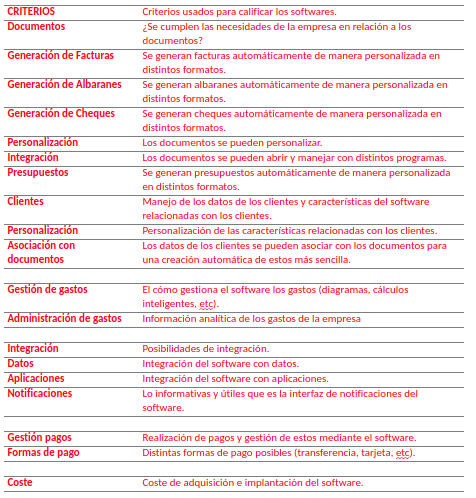
\includegraphics[scale=0.6]{images/tabla.png}
\end{center}

\begin{itemize}
\item \textcolor{Red}{Trebede\\}
\textcolor{Red}{\textbf{Documentos:}}
\begin{itemize}
\item \textcolor{Red}{\textbf{Generación de Facturas:} Hay un módulo completo dedicado a la facturación, que maneja los informes, los impuestos, periodicidad de facturas, automatización, etc.}
\item \textcolor{Red}{\textbf{Generación de Albaranes:} No hay información.} 
\item \textcolor{Red}{\textbf{Generación de Cheques:} No hay información.} 
\item \textcolor{Red}{\textbf{Personalización:} En el módulo de facturas hay funcionalidades de personalización.}
\item \textcolor{Red}{\textbf{Integración:} Sin especificar.} 
\item \textcolor{Red}{\textbf{Presupuestos:} Crear presupuestos, manejo de datos y creación de informes.}
\end{itemize}
\textcolor{Red}{\textbf{Clientes:}}
\begin{itemize}
\item \textcolor{Red}{\textbf{Personalización:} Hay campos personalizados para las fichas de los clientes, relacionados la necesidad de información según el tipo de negocio.} 
\item \textcolor{Red}{\textbf{Asociación con documentos:} Se pueden adjuntar documentos de cualquier tipo y almacenarlos en la ficha del cliente.}
\end{itemize}
\textcolor{Red}{\textbf{Gestión de gastos:} Administración de gastos: Hay una herramienta de administración de gastos personalizable que permite anotar tanto gastos sencillos como complejos con posibilidad de exportación del informe.\\}
\textcolor{Red}{\textbf{Integración:} No viene bien especificado.\\}
\textcolor{Red}{\textbf{Notificaciones:} Se pueden configurar Alarmas. Hay recordatorios de agenda mediante correo electrónico.\\}
\textcolor{Red}{\textbf{Gestión pagos:} Formas de pago: No especificado.\\}
\textcolor{Red}{\textbf{Coste:} El coste de adquisión de Trebede es de 15 euros por usuario y por mes. Suponemos que el software solo será utilizado por el departamento de Gestión Comercial, por tanto, el coste sería de 15 (1 usuario que es el departamento) por 12 meses, que daría un total de 180 euros al año.}
\item \textcolor{Red}{Factusol\\}
\textcolor{Red}{\textbf{Documentos:}}
\begin{itemize}
\item \textcolor{Red}{\textbf{Generación de Facturas:} Se generan facturas y facturas electrónicas.}
\item \textcolor{Red}{\textbf{Generación de Albaranes:} Disponible.}
\item \textcolor{Red}{\textbf{Generación de Cheques:} No Disponible.} 
\item \textcolor{Red}{\textbf{Personalización:} Hay posibilidad de personalización en el precio (ofertas) y diseño de informes.}
\item \textcolor{Red}{\textbf{Integración:} Los documentos se pueden exportar en PDF, pptx, Excel, OpenOffice, etc. Por tanto, los softwares que usa actualmente la empresa para trabajar con documentos, los puede seguir utilizando si se implantase Factusol.} 
\item \textcolor{Red}{\textbf{Presupuestos:} Disponible y personalizable.}
\end{itemize}
\textcolor{Red}{\textbf{Clientes:} La funcionalidad de clientes está disponible solo para temas de Almacén, que esta empresa no aborda.}
\textcolor{Red}{\textbf{Gestión de gastos:}}
\begin{itemize}
\item \textcolor{Red}{\textbf{Administración de gastos:} Previsión de pagos, previsión de cobros, estados de cobros y pagos, consumos y resúmenes mensuales, etc.}
\item \textcolor{Red}{\textbf{Integración:} Importar datos desde Excel, OpenOffice, Factuaplus, etc para la creación de informes. Mensajes SMS/MMS.}
\end{itemize}
\textcolor{Red}{\textbf{Notificaciones:} Email, SMS/MMS, calendario, agenda, etc.\\}
\textcolor{Red}{\textbf{Gestión pagos:} Formas de pago: Disponible.\\}
\textcolor{Red}{\textbf{Coste:} El coste de adquisición de Factusol depende de la versión del software que se decida adquirir. Como las necesidades de la empresa no son excesivamente altas, hemos optado por la versión estándar, que cuesta 195€ al año y tiene un soporte técnico aceptable.}
\end{itemize}
\end{itemize}

\textcolor{Red}{\texbf{Modelo de Calificación resultante:}}

\begin{center}
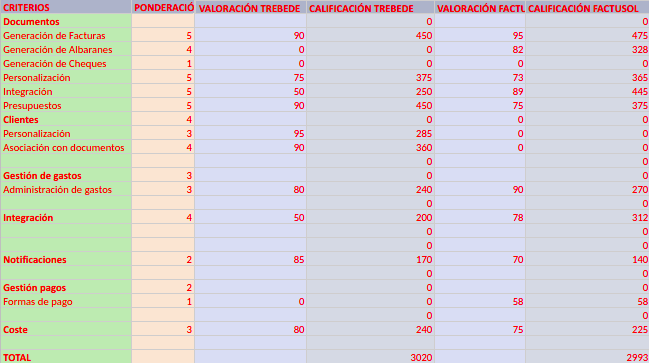
\includegraphics[scale=0.5]{images/calif.png}
\end{center}

\textcolor{Red}{Según el modelo de calificación, el software ganador es Trebede con una calificación de 3020, frente a una calificación de 2993 de Factusol. Las calificaciones son similares, por lo que se puede decir que, a la hora de elegir los softwares, se han elegido dos que cumplen más o menos los requisitos necesarios de manera equivalente.}

\textcolor{Red}{\subsubsection{\textbf{Modelo de coste de propiedad para Sistemas de Gestión Comercial}}}

\textcolor{Red}{La empresa que nos encontramos analizando utiliza un programa que es Trello para gestión de documentos, proyectos e intercomunicación entre los departamentos (mayoritariamente para proyectos), organizando los flujos de trabajo y gestionando tareas. Pero ningún sistema de información dedicado al almacenaje de documentos de forma permanente de manera electrónica. También utiliza las distintas funcionalidades que proporciona un sistema operativo. Por ello, sería conveniente analizar si implantar un sistema de gestión documental y/o archivo electrónico sería una buena opción para la empresa. O con lo que ya tiene la empresa basta e incluir tan solo archivo electrónico. Aunque sea una empresa pequeña y no tiene necesidad de comprar un software para gestionar documentos, puede que necesite guardar archivos de forma permanente y bien organizada, ya sea facturas, albaranes, cheques, o proyectos que se hicieron y finalizaron y no existe necesidad de reciclaje.} 

\begin{itemize}
\item \textcolor{Red}{Trebede}
\begin{center}
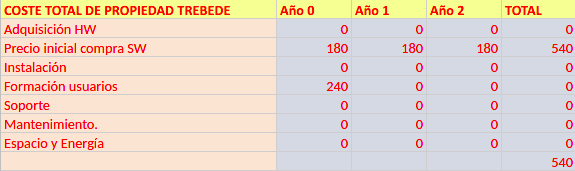
\includegraphics[scale=0.5]{images/trebede.png}
\end{center}
\textcolor{Red}{El coste total de propiedad de Trebede es de 540 euros.}
\item \textcolor{Red}{Factusol}
\begin{center}
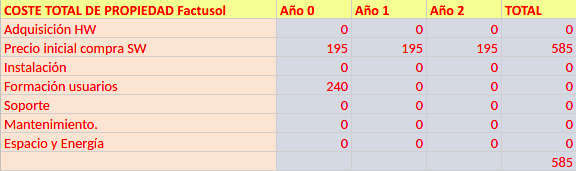
\includegraphics[scale=0.5]{images/factusol.png}
\end{center}
\textcolor{Red}{El coste total de propiedad de Factusol es de 585 euros.}
\end{itemize}

\textcolor{Red}{\textbf{Cambios que implicaría en la organización implantar la opción ganadora}}

\textcolor{Red}{Si se implantase la opción ganadora, tanto en el modelo de calificación como resultado más barato en el modelo de coste de propiedad, se prevén beneficios.} 

\textcolor{Red}{Respecto a la formación de usuarios, implica un coste, pero es bastante asequible teniendo en cuenta el ahorro de tiempo que implica la automatización de factura, presupuestos y posibles informes que se necesitarán. Como la herramienta es sencilla de manejar, y solo hay que dedicarle tiempo, y además, solo un departamento la utilizaría, el tiempo de implantación sería corto, ya que no se necesita ningún hardware nuevo y los equipos con los que cuenta la empresa soportan Trebede, por tanto, el tiempo de implantación depende solamente de la formación de usuarios. Trebede, al tratarse de un software relativamente sencillo, no cuenta con muchas integraciones, pero no es algo que vaya a entorpecer el uso del software, ya que solo se necesita poder usarlo con Microsoft Office y  PDF. Los datos e información de la empresa no presentarán ningún cambio a la hora de implantar el software, en cualquier caso, solo aumentaría la información por la base de datos de clientes que tiene Trebede. En resumen, a un pequeño coste adicional, se conseguirá un ahorro de tiempo a largo plazo por la automatización de una tarea que hasta ahora, se ha hecho a mano.}

\begin{itemize}
\item \textcolor{Red}{\textbf{\subsubsection{\textcolor{Red}{Almacén}}:} La empresa sobre la que se habla en este informe no comercia con productos ni artículos, ni online ni físicamente, ni tiene ningún almacén, por tanto, no se puede realizar ningún análisis que pueda resultar una mejora o innovación para la empresa en relación a los sistemas de información de gestión de almacenes.}
\item \textcolor{Red}{\textbf{\subsubsection{\textcolor{Red}{Comercio electrónico}}:} Actualmente no está disponible este servicio en esta empresa, ya que la página web que tienen es meramente corporativa e informativa. En el supuesto caso de que existiera y tuvieran una tienda online por la que los clientes pudieran contratar los servicios que ellos ofertan mediante esa vía, el departamento de programación serían los encargados del correcto mantenimiento y funcionamiento de la página mediante el uso de HTML5, JQuery, SQL y cualquier plugin necesario para la implementación y automatización de pagos, tanto para B2B como B2C.}
\textcolor{Red}{Esto agilizaría en gran medida las ventas de la empresa, ya que no siempre se vería obligado el Dpto. Marketing y Ventas a tener que hablar presencialmente con cada uno de los clientes para la formalización de un nuevo contrato. Así   pues, creemos que es una medida que deberían de implantar ya que es precisamente lo mismo que ellos ofertan a sus clientes, poder abrirse al mercado laboral mediante las nuevas tecnologías, pero ellos no terminan de implantar esto mismo en su empresa.}
\begin{center}
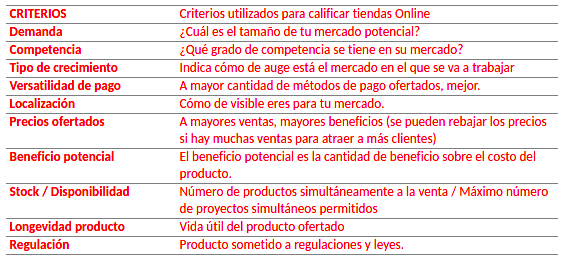
\includegraphics[scale=0.5]{images/online.png}
\end{center}

\textcolor{Red}{\textbf{SIN TIENDA ONLINE:}}
\begin{itemize}
\item \textcolor{Red}{\textbf{Organización:}}
\begin{itemize}
\item \textcolor{Red}{\textbf{Demanda:} El tope existirá allí donde el boca-boca del cliente que ya ha trabajado con la empresa no llega.}
\item \textcolor{Red}{\textbf{Competencia:} Muy alta.}
\item \textcolor{Red}{\textbf{Tipo de crecimiento:} Muy bajo dada su poca visibilidad.}
\item \textcolor{Red}{\textbf{Localización:} Únicamente de forma física y presencial en la oficina.}
\item \textcolor{Red}{\textbf{Versatilidad de pago:} Efectivo ó transferencia bancaria. }
\end{itemize}
\item \textcolor{Red}{\textbf{Gestión de gastos:}}
\begin{itemize}
\item \textcolor{Red}{Precios Ofertados: Los acordados en cada una de las entrevistas presenciales}
\item \textcolor{Red}{Beneficio Potencial: El necesario para que el proyecto salga rentable.}
\end{itemize}
\item \textcolor{Red}{\textbf{Conservación:}}
\begin{itemize}
\item \textcolor{Red}{Stock / Disponibilidad: Tantos proyectos como programadores en la empresa (a veces incluso se crea un cuello de botella y se conceden varios proyectos simultáneos)}
\item \textcolor{Red}{Longevidad: Cada proyecto tiene un período de vida de 1 año.}
\item \textcolor{Red}{Regulación: Cada proyecto está regulado según las leyes de cada país poseedor de la página que se le brinde.}
\end{itemize}
\end{itemize}

\textcolor{Red}{\textbf{TIENDA ONLINE:}}
\begin{itemize}
\item \textcolor{Red}{\textbf{Organización:}}
\begin{itemize}
\item \textcolor{Red}{\textbf{Demanda:} Tanta como visibilidad se le quiera dar en las redes}
\item \textcolor{Red}{\textbf{Competencia:} Bastante baja}
\item \textcolor{Red}{\textbf{Tipo de crecimiento:} Muy alto gracias al grosor de clientes.}
\item \textcolor{Red}{\textbf{Localización:} Cualquier parte del mundo.}
\item \textcolor{Red}{\textbf{Versatilidad de pago:} Todos los que el cliente desee.}
\end{itemize}
\item \textcolor{Red}{\textbf{Gestión de gastos:}}
\begin{itemize}
\item \textcolor{Red}{Precios Ofertados: Dependiendo de la ley de oferta y demanda.}
\item \textcolor{Red}{Beneficio Potencial: En base al anterior apartado.}
\end{itemize}
\item \textcolor{Red}{\textbf{Conservación:}}
\begin{itemize}
\item \textcolor{Red}{Stock / Disponibilidad: Tantos proyectos como programadores en la empresa (a veces incluso se crea un cuello de botella y se conceden varios proyectos simultáneos)}
\item \textcolor{Red}{Longevidad: Cada proyecto tiene un período de vida de 1 año.}
\item \textcolor{Red}{Regulación: Cada proyecto está regulado según las leyes de cada país poseedor de la página que se le brinde.}
\end{itemize}
\end{itemize}

\begin{center}
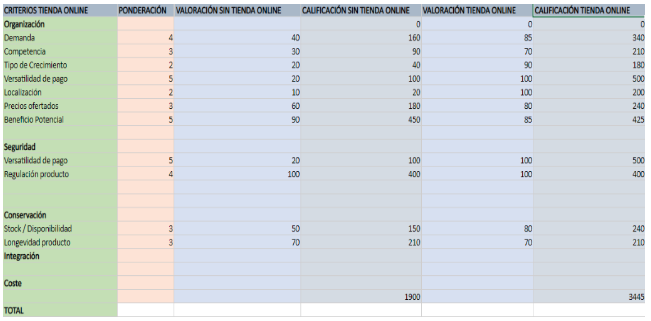
\includegraphics[scale=0.5]{images/tienda.png}
\end{center}

\textcolor{Red}{\textbf{Cambios que implicaría implantar la opción ganadora:}}
\textcolor{Red}{El coste de adquisición de una tienda Online tendría un coste monetario de 0 € dado que serían los mismos programadores de la empresa los encargados de realizar dicha página. Sólo habría que tener en cuenta el tiempo que desempeñarían en hacer dicha tienda visible y operativa al mundo, dado que mientras tanto otros proyectos se verían entorpecidos o suspendidos temporalmente. Luego, tras una pequeña inversión inicial de tiempo, se podría disponer de una herramienta de ventas potentísima que propulsaría la empresa seguramente a otro nivel adquisitivo.}
\item \textcolor{Red}{\textbf{\subsubsection{\textcolor{Red}{CRM}}} Hemos notado que la empresa utiliza bastantes softwares distintos (Business Facebook, Trello, Google Adds, etc.) en cada departamento y que la empresa podría utilizar un solo CRM que tiene las funcionalidades de casi todos los Sistemas de Información que se utilizan actualmente en la empresa. Para ello, vamos a crear un modelo de calificación y coste para tres CRMs distintos para poder tomar una decisión. Hemos elegido la opción de adquisión  porque es más rentable que desarrollar, ya que no se dispone de personal especializado en desarrollo de Sistemas de Información.} 
\end{itemize}

Hemos notado que la empresa utiliza bastantes softwares distintos (Business Facebook, Trello, Google Adds, etc.) en cada departamento y que la empresa podría utilizar un solo CRM que tiene las funcionalidades de casi todos los Sistemas de Información que se utilizan actualmente en la empresa. Para ello, vamos a crear un modelo de calificación y coste para tres CRMs distintos para poder tomar una decisión. 

Los CRMs que hemos elegido son: \textbf{holded CRM}, \textbf{SugarCRM} y \textbf{Microsoft Dynamics CRM}. 

Para el \textbf{modelo de calificación} se han tenido en cuenta los siguientes criterios: 

\begin{table}[H]
\begin{tabular}{l|l}
\hline
\textbf{Dashboard}  & \textbf{Calidad del significado visual de la dashboard} \\ \hline
Organización & Organización de la información que se muestra. \\ \hline
Obtención de los datos & Lo bien o mal que recoge los datos es SI.  \\ \hline
Coherencia & La coherencia de los datos recogidos.  \\ \hline
\textbf{Procesamiento de datos} & Acumulación y manipulación de los datos \\ \hline
Tratamiento de la ambigüedad & A la hora de procesar los datos, el manejo de la ambigüedad. \\ \hline
Precisión & Precisión con la que se procesan los datos (clasificación, etc.). \\ \hline
Integridad & Integridad de los datos antes y después de procesar. \\ \hline
Tratamiento de la información & Información obtenida tras procesar los datos. \\ \hline
Creación de documentos & \begin{tabular}{@{}c@{}}Con la información obtenida de los datos, la \\capacidad de generar documentos automáticamente.\end{tabular} \\ \hline
Integración con BD existente & \begin{tabular}{@{}c@{}}La capacidad del SI de modificar la base \\de datos en función a nueva información.\end{tabular} \\ \hline
Funcionalidad & Funcionalidad del CRM. \\ \hline
Idiomas & Idiomas que tiene disponible el CRM. \\ \hline
Perfiles de usuario & Posibilidad de personalización de los usuarios (permisos, perfiles, etc.). \\ \hline
Personalización & Posibilidad de personalización del software. \\ \hline
Sistema de soporte & Al adquirir el CRM, la calidad del soporte del software. \\ \hline
Diagnóstico de errores & Si el software tiene un error, la calidad del diagnóstico de este. \\ \hline
Solución de errores & En caso de error, eficiencia de la solución. \\ \hline
Disponibilidad & \begin{tabular}{@{}c@{}}Si hay cualquier duda o problema con el software, la \\disponibilidad del soporte para contactar y obtener respuesta.\end{tabular} \\ \hline
Actualizaciones & Periodo y calidad de las actualizaciones de software. \\ \hline
Guía del Sistema & \begin{tabular}{@{}c@{}}La calidad de la información proporcionada \\por la guía del software adquirido.\end{tabular} \\ \hline
Búsqueda de soluciones/dudas & \begin{tabular}{@{}c@{}}La guía tiene un buscador y este es eficiente \\para encontrar la información que se busca.\end{tabular} \\ \hline
FAQ & \begin{tabular}{@{}c@{}}Hay un foro en el cual interactúan los usuarios y desarrolladores \\en el cual se pueden observar las preguntas más frecuentes. \end{tabular} \\ \hline
Accesibilidad & Posibilidad de acceso al máximo de personas. \\ \hline
Limitaciones físico/sensoriales & \begin{tabular}{@{}c@{}}Para los usuarios con limitaciones físicas o \\sensoriales, el software es accesible sin problema.\end{tabular} \\ \hline
Limitaciones tecnológicas & \begin{tabular}{@{}c@{}}Por ejemplo, para los usuarios que se encuentren en una situación \\en la cual no pueden usar un dispositivo, que el software \\se pueda usar con otro dispositivo. También influye la \\posibilidad del uso del software con y sin conexión.\end{tabular} \\ \hline
Coste & Precio del software. \\ \hline         
\end{tabular}
\end{table}

\textbf{Análisis de los criterios} en función a cada software:

\begin{itemize}
\item \textbf{Holded CRM}
\begin{itemize}
\item \textbf{Dashboard:} 
\begin{itemize}
\item Organización: La dashboard muestra la información de manera organizada, aunque no tiene muchas novedades. Es parecida a los demás CRMS. 
\end{itemize}
\item \textbf{Obtención de los datos:}
\begin{itemize}
\item Coherencia: Hay herramientas para importar datos. 
\end{itemize}
\item \textbf{Procesamiento de datos:}
\begin{itemize}
\item Tratamiento de la ambigüedad: Ninguna herramienta o característica relevante. 
\item Precisión: Suficiente.          
\item Integridad: Amazon, Shopify, paypal, Woocommerce, Dropbox, Google Drive, etc.
\end{itemize}
\item \textbf{Tratamiento de la información:}
\begin{itemize}
\item Creación de documentos: Creación ilimitada de facturas. 
\item Integración con BD existente: Posible. 
\end{itemize}
\item \textbf{Funcionalidad:}
\begin{center}
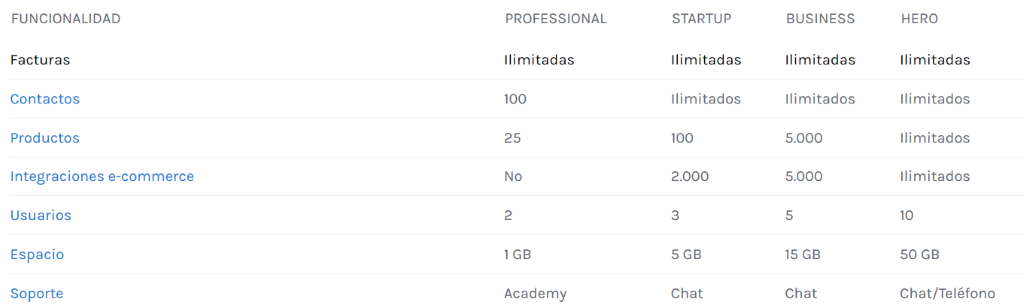
\includegraphics[scale=0.5]{images/func1.png}
\end{center}
\begin{itemize}
\item Idiomas: No especificado. 
\item Perfiles de usuario: Adaptado y personalizable. 
\item Personalización: Bastante personalizable.
\end{itemize}
\item \textbf{Sistema de soporte:}
\begin{itemize}
\item Diagnóstico de errores: No hay información. 
\item Solución de errores: Eficiente.         
\item Disponibilidad: Depende de la versión es más disponible o menos. Pero tiene buena disponibilidad. 
\item Actualizaciones : No hay información.
\end{itemize}
\item \textbf{Guía del Sistema:}
\begin{itemize}
\item Búsqueda de soluciones/dudas: Academy (Buscador, interacción entre usuarios y desarrolladores, publicación de soluciones). 
\item FAQ: Academy
\end{itemize}
\item \textbf{Accesibilidad:}
\begin{itemize}
\item Limitaciones físico/sensoriales: No existe. 
\item Limitaciones tecnológicas:  Se puede usar en cualquier dispositivo. 
\end{itemize}
\item \textbf{Coste:} Si elegimos la versión que pueden usar 5 usuarios (un usuario por departamento), serían 50 euros al mes, con pago anual.
\item \textbf{Casos de éxito:} Tres empresas, visionario, crepes y Texas y Verse
\end{itemize}
\item SugarCRM
\begin{itemize}
\item \textbf{Dashboard:} 
\begin{itemize}
\item Organización: La dashboard muestra la información de manera organizada, aunque no tiene muchas novedades. Es parecida a los demás CRMS.  
\end{itemize}
\item \textbf{Obtención de los datos:}
\begin{itemize}
\item Coherencia: Como los demás CRMs, tiene herramientas para importar y tratar esos datos importados, mediante archivos o Bases de Datos, etc. Aunque también se puede crear una BD nueva. 
\end{itemize}
\item \textbf{Procesamiento de datos:}
\begin{itemize}
\item Tratamiento de la ambigüedad:  Ninguna característica relevante, tratado por la herramienta BD que esté por debajo. 
\item Precisión: Suficiente. 
\item Integridad: Sin información suficiente.
\end{itemize}
\item \textbf{Tratamiento de la información:}
\begin{itemize}
\item Creación de documentos: A partir de la BD crea los documentos que se necesiten. 
\item Integración con BD existente: Bueno.
\end{itemize}
\item \textbf{Funcionalidad:}
\begin{itemize}
\item Idiomas: Existen módulos para añadir idiomas a la plataforma. 
\item Perfiles de usuario: Gran posibilidad de personalización de perfiles. 
\item Personalización: Muy  personalizable. 
\end{itemize}
\item \textbf{Sistema de soporte:}
\begin{itemize}
\item Diagnóstico de errores: Hay un soporte de usuario al cual se puede contactar y diagnosticarán el error, si existe. 
\item Solución de errores: Hay un soporte de ayuda para solucionar el problema.   
\item Disponibilidad: Buena disponibilidad durante las horas activas de la empresa. 
\item Actualizaciones : Cada x tiempo hay una actualización del CRM. 
\end{itemize}
\item \textbf{Guía del Sistema:}
\begin{itemize}
\item Búsqueda de soluciones/dudas: Existe una página de soporte con una guía de usuario y dudas resueltas. Y una comunidad de suaurios. 
\item FAQ: Disponible.
\end{itemize}
\item \textbf{Accesibilidad:}
\begin{itemize}
\item Limitaciones físico/sensoriales: Sin información. 
\item Limitaciones tecnológicas:  Multiplataforma. 
\end{itemize}
\begin{center}
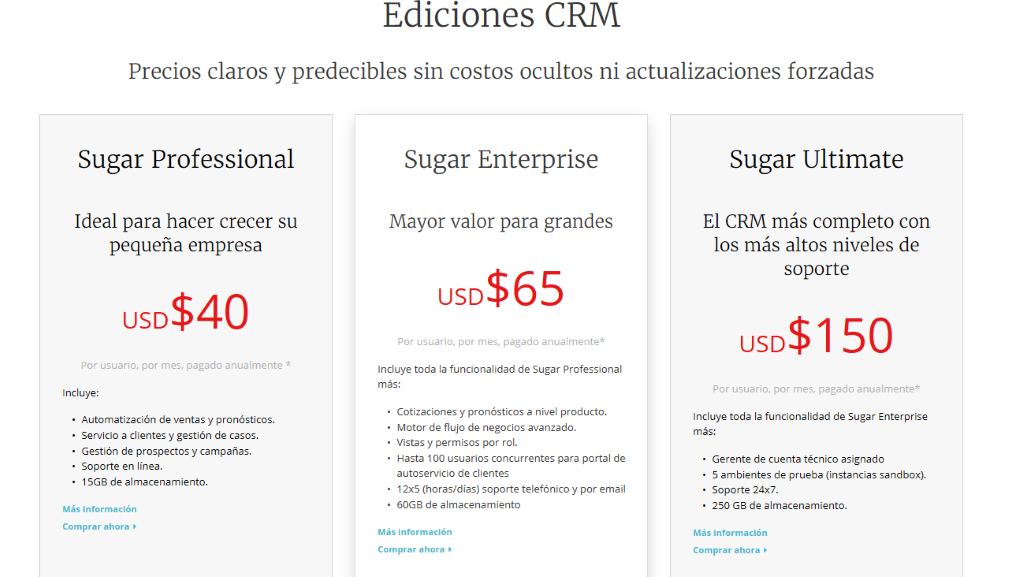
\includegraphics[scale=0.5]{images/coste.png}
\end{center}
\item \textbf{Coste:} Nuestra empresa con la versión profesional estaría bien. El coste sería de 35 euros por usuario y por mes, pagado anualmente. Bastante más alto que Holder CRM.
\item \textbf{Casos de éxito:} IBM, Uship.
\end{itemize}
\item Microsoft Dynamics CRM
\begin{itemize}
\item \textbf{Dashboard:}
\begin{center}
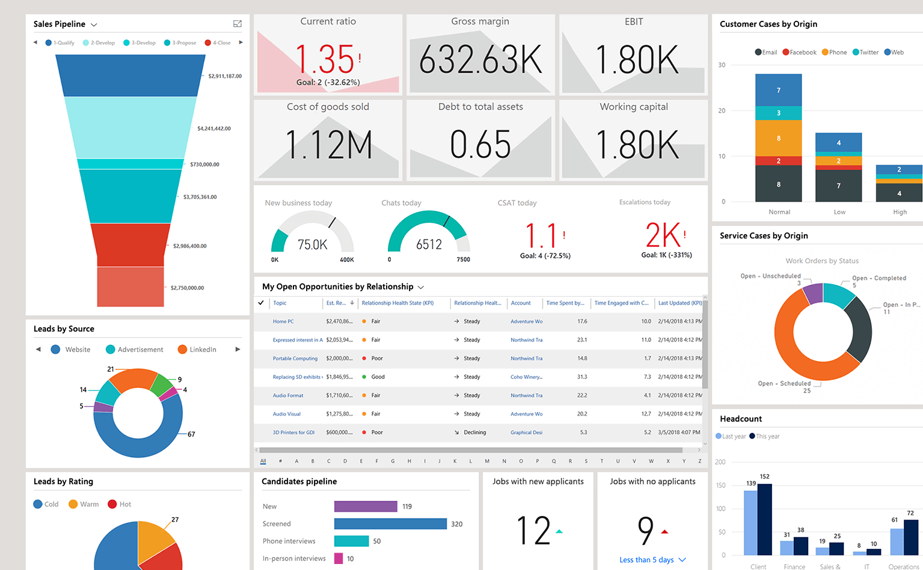
\includegraphics[scale=0.5]{images/dashboard.png}
\end{center}
\begin{itemize}
\item Organización: La dashboard de este CRM es similar a las demás, aunque la organización es un poco más intuitiva. 
\end{itemize}
\item \textbf{Obtención de los datos:}
\begin{itemize}
\item Coherencia: Existen herramientas que permiten importar datos de manera coherente, como son Import data Wizard. 
\end{itemize}
\item \textbf{Procesamiento de datos:}
\begin{itemize}
\item Tratamiento de la ambigüedad: Normal, ninguna característica relevante para este problema. 
\item Precisión: Suficiente. 
\item Integridad: Integridad con todos los software de Microsoft (Outlook, Windows 10, etc).
\end{itemize}
\item \textbf{Tratamiento de la información:}
\begin{itemize}
\item Creación de documentos: Genera los documentos que se necesiten en formato PDF. 
\item Integración con BD existente: Bueno.
\end{itemize}
\item \textbf{Funcionalidad:}
\begin{itemize}
\item Idiomas: Se pueden habilitar los paquetes de idiomas. 
\item Perfiles de usuario: Posibilidad de crear usuarios con distintos roles. 
\item Personalización: Se puede personalizar. 
\end{itemize}
\item \textbf{Sistema de soporte:}
\begin{itemize}
\item Diagnóstico de errores: Hay un sistema de soporte al que se le pueden poner tickets y ellos miran el problema o se puede contactar directamente con ellos. 
\item Solución de errores: En el momento en el que los técnicos del sistema de soporte leen el ticket o reciben una consulta, se encargan de solucionar el problema.          
\item Disponibilidad: Buena disponibilidad durante el horario activo de la empresa. 
\item Actualizaciones : Actualizaciones periódicas. 
\end{itemize}
\item \textbf{Guía del Sistema:}
\begin{itemize}
\item Búsqueda de soluciones/dudas: Hay un foro en el que se pueden preguntar dudas o buscar dudas resueltas. 
\item FAQ: Existe un foro con preguntas frecuentes bastante completo. 
\end{itemize}
\item \textbf{Accesibilidad:}
\begin{itemize}
\item Limitaciones físico/sensoriales: Tiene control para las discapacidades (como métodos abreviados de teclado) en temas de accesibilidad. 
\item Limitaciones tecnológicas: Multiplataforma, local, online. 
\end{itemize}
\item \textbf{Coste:} Al ser una empresa pequeña o mediana, con la versión básica de Microsoft Dinamics 365 valdría. Son 101€ por usuario y al mes, con pago anual, bastante más caros que las otras versiones analizadas. 
\begin{center}
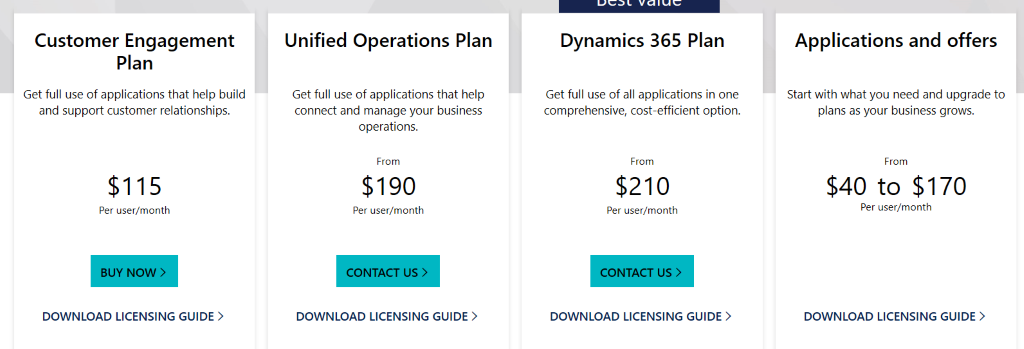
\includegraphics[scale=0.5]{images/costes.png}
\end{center}
\item \textbf{Casos de éxito:} Bastantes, entre ellos, Siemens, Fridays y Macys.
\end{itemize}
\end{itemize}

Los parámetros de ponderación escogidos han sido del 1 al 7, ya que hay un amplio abanico de criterios sobre los que calificar con distintas importancias. 

El modelo de calificación obtenido nos ha dado una calificación de 6950 para holder CRM, 7060 para Sugar CRM y 7980 para Microsoft Dynamics 365. Las calificaciones de los tres software han salido parecidas, pero finalmente la opción ganadora ha sido Microsoft Dynamics 365.

\begin{center}
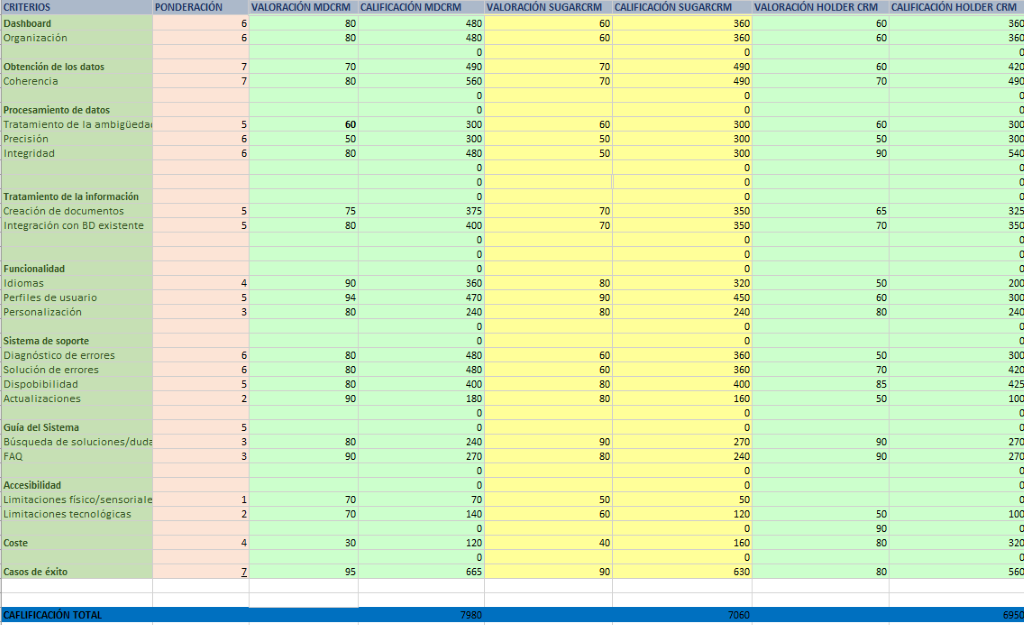
\includegraphics[scale=0.5]{images/ponderacion.png}
\end{center}

El modelo de calificación mostrado anteriormente se adjunta en formato “.excel” para futuras consultas o modificaciones. 

Para complementar la decisión de si adquirir un nuevo sistema de información o no, y en caso de implantarlo, elegir cuál, se ha creado un modelo de coste total de propiedad para calcular el coste a largo plazo de la implantación del nuevo software. 

\textbf{Coste total de propiedad}

\textbf{Criterios para calcular el coste de propiedad:}

\begin{center}
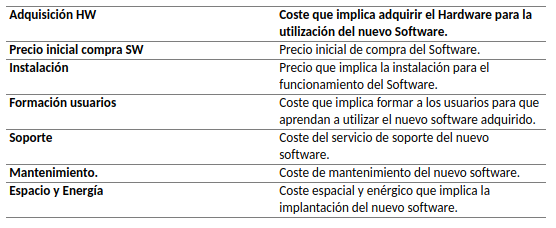
\includegraphics[scale=0.5]{images/costePropiedad.png}
\end{center}

\textbf{Calculo del Coste de la Propiedad}

\begin{center}
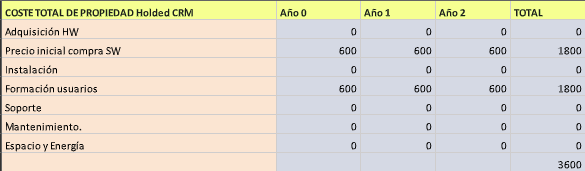
\includegraphics[scale=0.5]{images/Holded.png}
\end{center}

\begin{center}
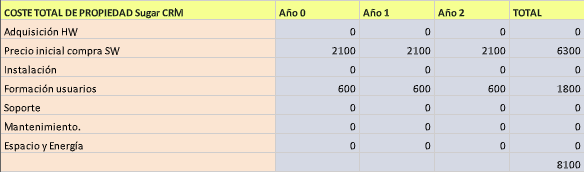
\includegraphics[scale=0.5]{images/sugar.png}
\end{center}

\begin{center}
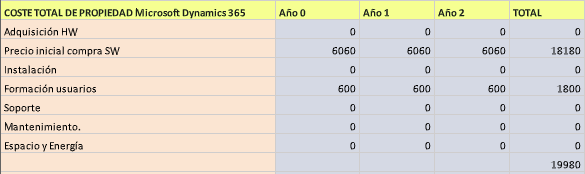
\includegraphics[scale=0.5]{images/Microsoft.png}
\end{center}

Observando los modelos de coste de propiedad creados, Microsoft Dynamics 365 es mucho más caro de los otros dos softwares. Holded CRM es notoriamente el más barato y Sugar CRM está en un lugar intermedio.

\vspace{5mm}

\textcolor{Red}{\textbf{\underline{Cambios que implicaría en la organización implantar la opción ganadora}}}

\vspace{5mm}

\textcolor{Red}{Actualmente la empresa tiene su manera de trabajar y al ser una empresa pequeña, funciona bien con los softwares que utiliza.  Respecto a la formación, un CRM al ser un software bastante completo y complejo de dominar, se necesitaría un formación personalizada de usuarios que implicaría un coste que no es rentable. Además, respecto al tiempo, según el cálculo, la formación sería de un mes, oficialmente, pero para que la empresa entera y todos los usuarios se acostumbren a usar el nuevo software y exista la misma fluidez que existía antes de implantar el software, pasaría bastante tiempo (entre medio año y un año), por lo que habría una pérdida de rendimiento durante una duración de tiempo que no conviene.}

\textcolor{Red}{El tiempo de implantación, si se incluye la formación de usuarios descrita anteriormente, sería bastante largo. Aunque realmente el tiempo que se tarda en instalar el software en los equipos de la empresa y migrar los datos no es mucho, ya que la parte complicada, que es migrar los datos, no costaría mucho ya que no es una gran cantidad de datos la que está en la base de datos de la empresa y en caso de querer integrar bases de datos, el CRM propuesto tiene una alta integración. } 

\textcolor{Red}{El software propuesto al tener integridad con varios servicios de Google, Microsoft, Amazon, plataformas de pago como Paypal, comercio electrónico, etc. es bastante conveniente. Pero en la empresa que estamos analizando, no se utiliza ningún software que se pueda integrar con Holded CRM, por ello, no es una gran ventaja. Si se comenzasen a utilizar los servicios que tienen integración con este CRM, entonces quizá ya sí sería una buena opción. }

\textcolor{Red}{Aunque la migración de datos y las integraciones con bases de datos ya existentes sea aparentemente buena, siempre existe el riesgo de perder datos o información. Para saber si esta pérdida sería significativa o no, habría que hacer un estudio de la información y datos de la que dispone la empresa y el formato en el que está guardada la información y ver si la pérdida sería significativa y si rentaría crear una base de datos nueva o no habría pérdida significativa y simplemente se migrarían los datos.}

\textcolor{Red}{Análisis y evaluación de aplicación a la empresa seleccionada de los siguientes sistemas de información:}

\subsubsection{\textcolor{Red}{Archivo electrónico}}

\textcolor{Red}{\textbf{CRITERIOS ARCHIVO ELECTRÓNICO}}
\begin{center}
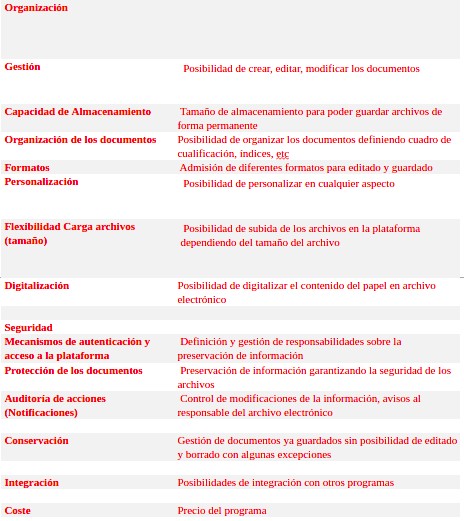
\includegraphics[scale=0.5]{images/earch.png}
\end{center}
\begin{itemize}
\item \textcolor{Red}{\textbf{Fedora:}}\\
\textcolor{Red}{\textbf{CRITERIOS ARCHIVO ELECTRÓNICO}}
\begin{center}
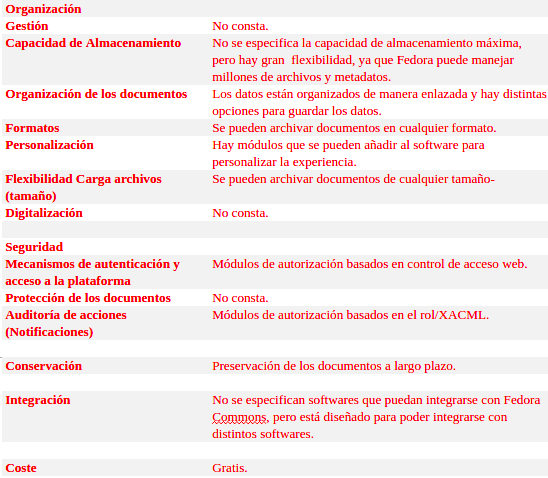
\includegraphics[scale=0.5]{images/earch2.png}
\end{center}
\item \textcolor{Red}{\textbf{ResourceSpace:}}\\
\textcolor{Red}{\textbf{CRITERIOS ARCHIVO ELECTRÓNICO}}
\begin{center}
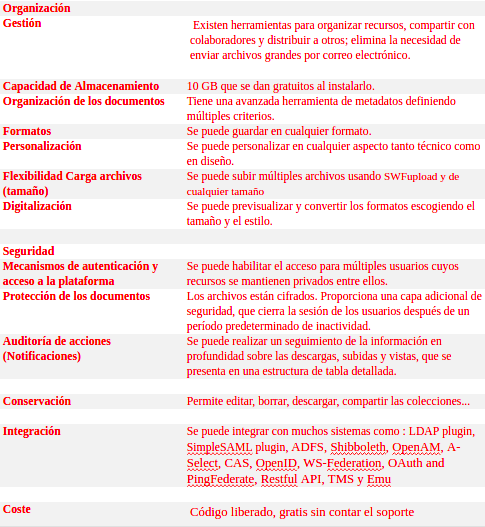
\includegraphics[scale=0.5]{images/earch3.png}
\end{center}
\end{itemize}

\subsubsection{\textcolor{Red}{Modelos}}

\textcolor{Red}{\textbf{Modelo de calificación resultante}}

\begin{center}
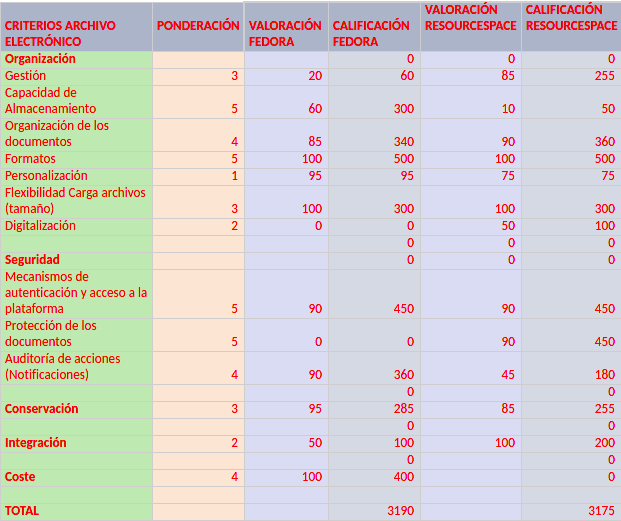
\includegraphics[scale=0.5]{images/calificaciones.png}
\end{center}

\textcolor{Red}{\textbf{Modelo de coste de propiedad}}

\begin{itemize}
\item \textcolor{Red}{Fedora}
\begin{center}
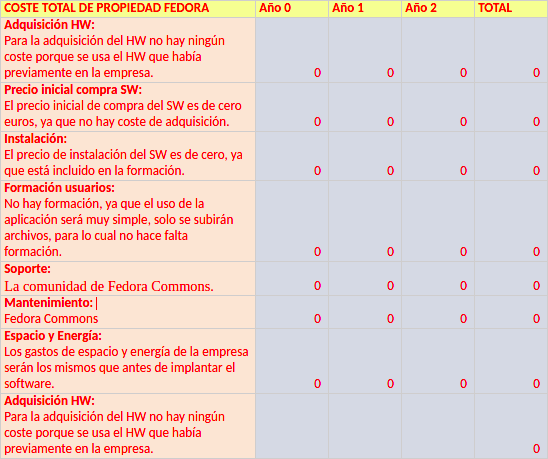
\includegraphics[scale=0.5]{images/fedora.png}
\end{center}
\textcolor{Red}{El coste total de propiedad de Fedora es de cero euros.}
\item \textcolor{Red}{ResourceSpace}
\begin{center}
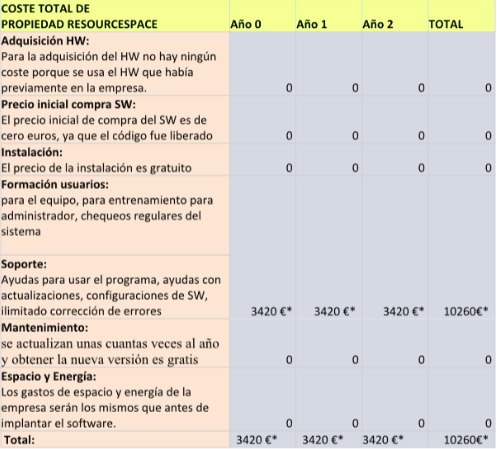
\includegraphics[scale=0.5]{images/rs.png}
\end{center}
\textcolor{Red}{Se puede contratar paquetes entre los cuales se puede elegir Virtual Cloud, Performance Cloud y Enterprise Cloud. El precio escogido es de paquete Virtual Cloud, que es un precio mínimo. Aparte de estos servicios mencionados arriba se incluyen más cosas como almacenamiento hasta 2TB (estamos hablando de tipo cloud), copias de seguridad sin redundancia geográfica. Se puede instalar el software sin servicio de soporte y sin formación de usuarios, sería arriesgado si surgiera cualquier problema con el programa. Aún así, en esta empresa tampoco es que haya mucha documentación que manejar y podría ser un gasto innecesario.}  

\textcolor{Red}{El coste total de propiedad de ResourceSpace es de 10260 euros.}
\end{itemize}

\section{Integración de sistemas: análisis y evaluación de su aplicación a la empresa seleccionada}

\textcolor{Red}{En el caso de gestión comercial hemos visto que en nuestro modelo de calificación el que mayor puntuación obtuvo fue Trebede, ya que sería una manera electrónica, sencilla y con las necesidades que pudiera tener la empresa, para la correcta manipulación de pagos, recibos, etc. Actualmente la empresa es demasiado pequeña como para tener que plantearse la instalación de dicho software, así que a día de hoy, aunque sea la opción ganadora del modelo de calificación, no es necesaria en estos momentos.}

\textcolor{Red}{Para el caso del comercio electrónico suponemos que habría una clara y directa integración de funcionalidades entre el Departamento de Marketing, Programación y Diseño y Redes. Ya que, si acceden a la página, querrá decir que el Dpto. Redes ha hecho bien su trabajo, si el cliente navega por la web y le parece atractiva, que el Dpto Marketing lo hizo bien, si optan por elegir un diseño personalizado, querrá decir que el Departamento de Diseño también trabaja correctamente y, si están conformes con el precio y con el objeto final, que tanto la parte contable como el Departamento de Programación han funcionado correctamente. Así pues únicamente la implementación de esta opción requerirá una inversión de tiempo, que conllevará una mejor unificación de prácticamente todos los departamentos, agilizando el proceso de comunicación y trabajo con el cliente, así pues de ofrecerle una mayor información sobre sus proyectos, creándole así mayor tranquilidad en el proceso de creación de sus peticiones.}

\textcolor{Red}{Por el pequeño tamaño que tiene la empresa y el público que abarca, no tiene sentido de hablar de un CRM para integrar todos los sistemas que lo forman (Marketing, Programación, Diseño, Redes, etc), bastará con emular dicha funcionalidad a través de la plataforma Trello que ya utilizan, donde mediante tableros de actividades, pueden establecer pautas de trabajo, establecer fechas límite, crear, modificar y asignar nuevas tareas e informar en todo momento sobre lo que se hizo, se ha hecho o se va a hacer en el futuro, independientemente del departamento.}

\textcolor{Red}{Puede que en un futuro, cuando la empresa haya conseguido crecer lo suficiente que dicha emulación de CRM en dicha plataforma no sea suficiente y sea necesario tomar otras medidas, pero aún esa posibilidad no se visualiza ni a largo plazo, ya que la empresa no quiere crecer en cantidad de empleados, sino en calidad de los mismos.}

\section{Sistemas de flujo de Trabajo}

\begin{itemize}
\item Identificar y modelar los principales flujos de trabajo de la empresa
\end{itemize}
\textcolor{Red}{Los principales flujos de trabajo de la empresa son: La captación de clientes, la entrevista con los mismos, la creación de los diseños de sus productos, la creación de lo mismo y la entrega del producto finalizado.}

Diagramas en Bizagi a modo explicativo de algunas funcionalidades que desempeña la empresa: 

\begin{itemize}
\item Renovar un cliente
\begin{center}
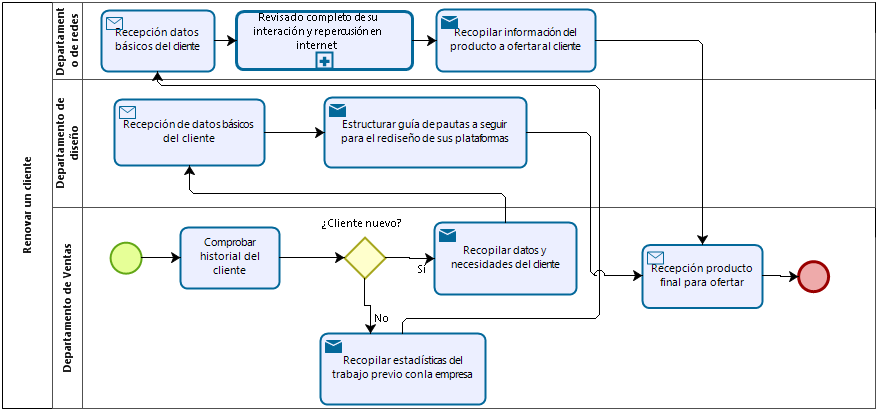
\includegraphics[scale=0.5]{images/cliente.png}
\end{center}
De manera sencilla podemos ver que el flujo de actividad de esta tarea la inicializa el departamento de ventas quien deberá llevar un historial de los posibles/futuros y actuales clientes, realizando actualizaciones periódicas sobre ellos (para ofrecerles nuevos productos o actualizar los que ya tengan). 

Dependiendo de si ya han trabajado previamente con la empresa o no, se recogerán todos los datos necesarios para generar los productos que necesite el cliente, en los márgenes y límites de tiempo establecidos y firmados mediante contratos.
\item Diseñar una página web
\begin{center}
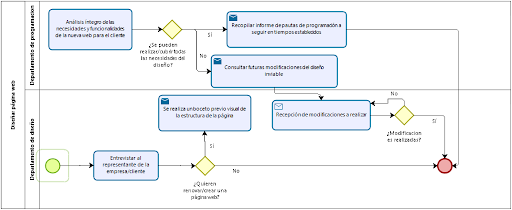
\includegraphics[scale=0.5]{images/web.png}
\end{center}
Para llevar acabo esta tarea será necesaria la comunicación entre el departamento de diseño y el departamento de programación, quiénes serán los encargados de dar el visto bueno final del proyecto. 

Primeramente, el Departamento de Diseño redactará una primera impresión de lo que será la página web que desee el cliente en función de una serie de entrevistas con él y de recopilar información. Una vez dicha información llegue al Departamento de Programación, ellos deberán ver si pueden poner en práctica, si es viable o tan siquiera si tiene sentido realizar todas las funcionalidades y maquetaciones que sugiere el Departamento de Diseño. Si todo funciona correctamente, se establecen los tiempos y fechas de entrega final y se daría comienzo a realizar dicha página, si por el contrario no fuera así, volvería el flujo de actividad sobre el Dpto. Diseño quién debería de rediseñar dicho proyecto para su óptimo funcionamiento.
\item Gestión de redes sociales
\begin{center}
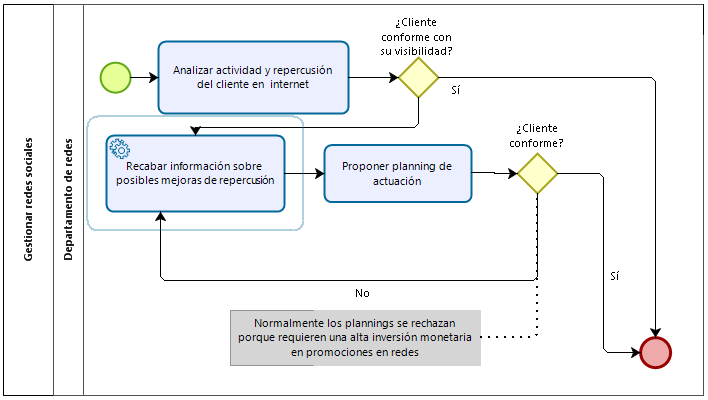
\includegraphics[scale=0.5]{images/rrss.png}
\end{center}
Dicho departamento se encargará de analizar mediante herramientas estadísticas y
promociones monetarias, la repercusión, el peso y el posicionamiento de las redes
de nuestro cliente. Si el cliente no está conforme con la situación actual, se le hará
un planning de actuación con respecto a la actividad que se programará para sus
redes, las promociones que tendrán y la repercusión que tendrá en base al público
que atraen, con el consecuente coste de llevar a cabo dicha campaña. Si el cliente lo
ve lógico y está conforme, dará paso al Dpto. A realizar dicha campaña, en caso
negativo, deberán crear un nuevo planning ó modificar el antíguo hasta lograr llegar
a un consenso.
\end{itemize}

\section{Propuestas innovadoras de Sistemas de Información para la Organización}

\textcolor{Red}{Como sabemos, la empresa que estamos analizando se dedica a hacer estrategias de publicidad a medida para los clientes, que normalmente es a nivel de web. Una propuesta, no tan innovadora, pero útil, sería utilizar un sistema de información que automatice la creación de páginas webs y que implemente módulos de publicidad, para los clientes que exijan menos personalización. Así se podría ahorrar un poco de trabajo a los programadores. }

\textcolor{Red}{Como se observó en el análisis de CRM, implantar uno no sería muy viable, sin embargo, una plataforma sencilla de gestión de clientes que incluya un portal de comunicación podría ser bastante útil, ya que la comunicación, que se realiza por email, pasaría de estar en hilos desorganizados a un sistema en el cual cada cliente tiene su propio hilo y los mensajes no están mezclados, o incluso un gestor de proyectos en el cual en cada proyecto el cliente pueda comunicarse con la empresa.}

\textcolor{Red}{Ya se he mencionado anteriormente, pero la implantación de una tienda online en la empresa sería de un gran beneficio, ya que restaría tiempo al departamento de ventas y marketing para entrevistar a sus potenciales clientes, cuando estos pueden elegir los productos que desean desde sus oficinas y hogares.}

\textcolor{Red}{Haciendo también una pequeña mención a cómo funcionan internamente las oficinas de Google, éste se encuentra en el ranking de las 100 mejores empresas en las que uno podría trabajar, ya que ofrecen servicios y facilidades para el empleado de todo tipo. Fijándonos en ellos y aplicándolo a nuestra empresa, otra propuesta innovadora sería tener la oportunidad de elegir el tipo de silla que más le guste al empleado, junto con un servicio de cafetería con comida sana, ya que entendemos que los trabajadores pasarán muchas horas en la oficina, sentados y probablemente no se alimenten bien. Eso a la larga les provocará ansiedad que, finalmente se traducirá en un mal aprovechamiento del potencial del trabajador. Así pues, si el trabajador puede estar cómodamente sentado todas las horas que dedique en la oficina y se brinda la oportunidad de poder estar bien alimentado, seguramente la productividad de éste aumente positivamente.}

\textcolor{Red}{En la línea de la propuesta anterior, también se podría ofrecer teletrabajo a los empleados, ya que eso proporcionaría mayor flexibilidad en el horario, lo que llevaría a una mayor felicidad y comodidad, y por lo tanto, a un potencial aumento de la productividad y de la calidad de los productos resultantes.}

\textcolor{Red}{Sería ideal tener un sistema ERP que integre todos departamentos, y no que sea una intercomunicación solo por Trello. Ahorraría mucho tiempo, lo que es una mejoría para el negocio.}

\textcolor{Red}{Respecto a la contabilidad, en esta empresa no se utiliza nada, podrían meter algún programa que gestione todo esto y que se integre con otros programas. Este programa más archivo electrónico, integración de ambos softwares para que haya un flujo de trabajo automatizado: se generan los documentos en el programa de contabilidad y que automáticamente se guarde en el programa de archivo electrónico dependiendo de condiciones que se impongan. Lo importante que esto sea automatizado sin que haya un trabajador encima de esto todo el rato. Lo mismo pasaría con la integración de otros programas con el archivo electrónico ya que en esta empresa los trabajadores no se dedican a archivar. Con esto todo aumentaría la organización de documentos.}

\section{División de Tareas entre los miembros del grupo}

Para la repartición de tareas hemos creado una tabla:

\begin{center}
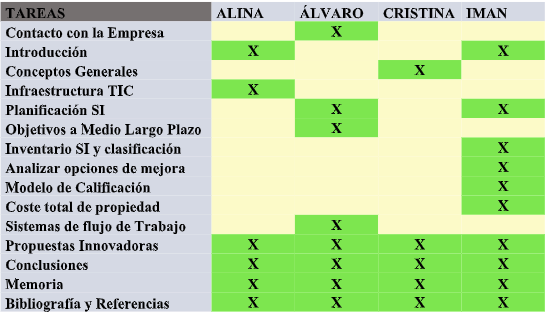
\includegraphics[scale=0.5]{images/tareas.png}
\end{center}

También hicimos otra para los cambios para mejorar la primera entrega:

\begin{center}
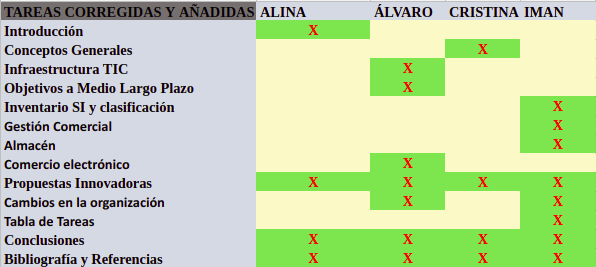
\includegraphics[scale=0.5]{images/cambios.png}
\end{center}

En la segunda entrega, la tabla pasa a ser la siguiente:

\begin{center}
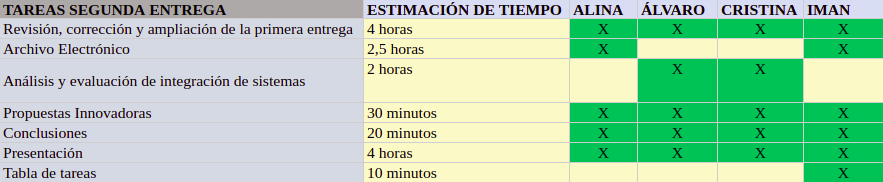
\includegraphics[scale=0.4]{images/tareas2.png}
\end{center}

\section{Conclusión}

\textcolor{Red}{Habiendo hecho un estudio del sistema de trabajo de la empresa, hemos llegado a la conclusión de que: }

\begin{itemize}
\item \textcolor{Red}{Tiene un sistema ya implantado y su propia manera de trabajar.}
\item \textcolor{Red}{Los planes para ampliar la plantilla y expandir la empresa son escasos, nulos prácticamente, ya que con la existente no hay sobrecarga para ningún trabajador, tampoco son excesivos y no hay problemas para pagar los sueldos. }
\end{itemize}

\textcolor{Red}{Partiendo de estos resultados, no se ve muy claro si realmente la empresa querría implantarlo, ya que habría que conocer muy bien la duración media de los trabajadores de la empresa y otros factores difíciles de conocer por personas ajenas a la empresa. }

\textcolor{Red}{Suponiendo que sí que se quisiera implantar Holded CRM, los cambios que habría que hacer serían más fáciles que si la empresa estuviera en proceso de expansión. Aun así, hay bastantes desventajas: }

\begin{itemize}
\item \textcolor{Red}{El proceso de adaptación al nuevo software se tendría que hacer igualmente, teniendo que acostumbrarse a una nueva forma de trabajo. }
\item \textcolor{Red}{Todos los proyectos que estaban llevándose a cabo se tendrían que migrar. }
\item \textcolor{Red}{Se tendría que plantear el cambio también en algunos softwares usados por la empresa a otros con los que Holded tiene muy buena integración. }
\end{itemize}

\textcolor{Red}{Aunque todo parezcan desventajas, también hay bastanes ventajas, y es que Holded CRM ofrece, a un precio bastante bueno, unas muy buenas condiciones de trabajo, y la integración con otros softwares que no son usados por la empresa, abriría la puerta a poder trabajar con software puntero desarrollado por empresas del sector como Google, Amazon y PayPal, entre otras.}

\begin{thebibliography}{9}

\bibitem{SisDir} \textit{Sistema Directivo}, \url{https://blogs.udima.es/administracion-y-direccion-de-empresas/libros/introduccion-a-la-organizacion-de-empresas-2/unidad-didactica-2-el-sistema-de-direccion-y-organizacion-principios-y-modelos-organizativos/1-introduccion-concepto-y-estructura-del-sistema-directivo/}.
\bibitem{SisFis} \textit{Sistema Físico}, \url{https://es.slideshare.net/yadithmartinezlopez5/trabajo-yadith}.
\bibitem{SisInf} \textit{Sistema de información}, \url{https://es.wikipedia.org/wiki/Sistema_de_informaci\%C3\%B3n}.
\bibitem{Sol} \textit{Soluciones CRM}, \url{https://www.dynamics-crm.es/soluciones-crm}.
\bibitem{Trello} \textit{Trello}, \url{https://trello.com/?truid=trf9bee6-b868-4daa-8024-85319ae8cb44}.
\bibitem{FacBus} \textit{Facebook Business}, \url{https://business.facebook.com/}.
\bibitem{Ads} \textit{Google Ads}, \url{https://ads.google.com/intl/es_es/start/?subid=es-es-adon-bi-aw-c-0-r0_xx_txx_xx_xx_bau_non!o2~350070004-\%7bcreative\%7d-kwd-77446954221687:loc-170&sourceid=awo&utm_source=aw&utm_medium=ha&utm_campaign=es-es-adon-bi-aw-c-0-r0_xx_txx_xx_xx_bau_non!o2~350070004-\%7bcreative\%7d-kwd-77446954221687:loc-170&utm_term=Google\%20Ads&utm_content=Desk\%2BTab\%20\%7C\%20AW\%20SEM\%20\%7C\%20BKWS\%20\%7C\%20EXA\%20~\%20\%5BWE\%5D\%20ES_ES_EXA_R0_\%5B1\%3A1\%5D\%20google\%20ads_xx_xx_xx&gclid=CIGNwKq2pN8CFYaMhQodfcED2w}.
\bibitem{FacPix} \textit{Facebook Pixel}, \url{https://www.pixelsoftwares.com/}.
\bibitem{ImplCRM} \textit{Ejemplos de CRM}, \url{https://www.crmswitch.com/implementing-crm/six-crm-dashboard-examples/}.
\bibitem{Casos} \textit{Casos de éxito de Holded}, \url{https://www.holded.com/es/casos-de-exito-de-clientes-de-holded}.
\bibitem{SugarCRM} \textit{Sugar CRM}, \url{https://files.sugarcrm.com/resources/datasheets/sugar-professional-2016-05-20-es.pdf}.
\bibitem{Exportacion} \textit{Exportación de datos en Sugar CRM}, \url{http://www.tecnologiafacil.com/importacion-y-exportacion-masiva-de-datos-en-sugarcrm/}.
\bibitem{Winner} \textit{Business Choice Awards: CRM}, \url{http://sugarcrm-online.s3.amazonaws.com/misc/pcmag-business-choice-winner-2016-07-20.pdf}.
\bibitem{GesDoc} \textit{Gestión de documentos en Sugar CRM}, \url{https://www.connecting-software.com/gestion-de-documentos-sugarcrm-mas-efectiva/}.
\bibitem{Modulos} \textit{Modulos en Sugar CRM}, \url{http://rodriguezizquierdo.com/como-instalar-modulos-o-cambiar-idioma-en-sugarcrm-version-6-5-10-build-8716/}.
\bibitem{GesPro} \textit{Gestion de perfiles}, \url{https://bebeyond.es/gestion-de-perfiles-permisos-de-usuarios-crm/}.
\bibitem{SuppPlat} \textit{Plataformas soportadas por Sugar CRM}, \url{http://support.sugarcrm.com/Resources/Supported_Platforms/index.html}.
\bibitem{CasosExito} \textit{Casos de éxito de Sugar CRM}, \url{https://www.intelligencepartner.com/conoces-estos-casos-de-exito-con-sugarcrm/}.
\bibitem{DynamicCRM} \textit{How to Organize Dynamics CRM Documents in SharePoint}, \url{https://www.crmsoftwareblog.com/2018/02/organize-dynamics-crm-documents-sharepoint/}.
\bibitem{PaqIdioma} \textit{Instalar y habilitar un paquete de idioma}, \url{https://docs.microsoft.com/es-es/previous-versions/dynamicscrm-2016/deployment-administrators-guide/hh699736\%28v\%3dcrm.8\%29}.
\bibitem{Sec} \textit{Crear usuarios en Dynamics 365 (online) y asignar roles de seguridad}, \url{https://docs.microsoft.com/es-es/dynamics365/customer-engagement/admin/create-users-assign-online-security-roles}.
\bibitem{Supp} \textit{Soporte Dynamics 365}, \url{http://soportedynamics.com/servicios/soporte-dynamics-365/}.
\bibitem{Updates} \textit{Actualizaciones acumulativas para Microsoft Dynamics 365 local}, \url{https://support.microsoft.com/es-es/help/3142345/microsoft-dynamics-365-onpremise-cumulative-updates}.
\bibitem{FAQ} \textit{FAQ de la política de Actualización}, \url{https://docs.microsoft.com/en-us/dynamics365/get-started/faq-update-policy}.
\bibitem{Hist} \textit{Historias de clientes}, \url{https://dynamics.microsoft.com/es-es/customer-stories/}.
\textcolor{Red}{\bibitem{GestAlm} \textit{Sistema de Gestión de Almacenes}, \url{https://es.wikipedia.org/wiki/Sistema_de_gestión_de_almacenes}.}
\textcolor{Red}{\bibitem{GestCom} \textit{Gestión Comercial}, \url{https://www.gestiopolis.com/que-es-gestion-comercial/}.}
\textcolor{Red}{\bibitem{Fact} \textit{Especificaciones Factusol}, \url{https://www.sdelsol.com/factusol360/mas-informacion/}.}
\textcolor{Red}{\bibitem{Trebede} \textit{Funcionamiento de Trebede}, \url{https://www.programagestioncomercial.es/caracteristicas/}.}
\textcolor{Red}{\bibitem{RS} \textit{ResourceSpace}, \url{https://www.resourcespace.com/}.}
\end{thebibliography}

\end{document}